\documentclass{article} 

\usepackage{packages}

\usepackage{environments}

\usepackage{commands}
\usepackage{ wasysym }
\usepackage{svg}
\usepackage{cancel}
\usepackage{nicematrix}
\newcommand{\divides}{\mathrel{\raisebox{-0.2ex}{\vdots}}}

\usepackage{titlepage}

\setUDK{512.643}
% Выбрать одно из двух
\setToResearch
%\setToProgram
\setTitle{Общие соседи вершин в $k$-тотальном графе кольца матриц}

% Выбрать одно из трех:
% КТ1 -- \setStageOne
% КТ2 -- \setStageTwo
% Финальная версия -- \setStageFinal
\setStageFinal
%\setStageTwo
%\setStageFinal

\setGroup{233}
\setStudentSgn{
\includegraphics[scale=0.2]{подпись.png}}
\setStudent{М. А. Разуваев}
\setStudentDate{01.04.2025}
\setAdvisor{Максаев Артем Максимович}
\setAdvisorTitle{Доцент Факультета компьютерных наук / Департамента больших данных и информационного поиска, к. ф.-м. н.}
\setAdvisorAffiliation{ФКН НИУ ВШЭ}
\setAdvisorDate{}
\setGrade{}
\setAdvisorSgn{}
\setYear{2025}


\begin{document}

\makeTitlePage

\tableofcontents

\begin{abstract}
Задачи Linear Preserver Problems (LPP) состоят в определении всех линейных операторов, сохраняющих заданные функции или свойства на пространстве матриц. LPP имеет много приложений в различных областях математики и естественных наук. Первым результатом в этой теории считается результат Фробениуса, который получил описание линейных отображений матриц над полем комплексных чисел, сохраняющих определитель. Одним из важных обобщений стал результат Хуа о сохранении смежных матриц (ранг разности которых равен 1). Это тесно связано с изучением соответствующего графа, вершины которого — матрицы, а рёбрами соединяются те из них, ранг разности которых равен k. Такой граф будем называть $k$-тотальным графом кольца матриц. Цель проекта состоит в его изучении: в частности, в изучении общих соседей его вершин.
\end{abstract}
\keywords{LPP, $k$-тотальный граф, общие соседи, автоморфизм}
\section{Условные обозначения}
л.н.з. — линейно независимые векторы\\
л.з. — линейно зависимые векторы\\
$M_{m \times n} = M_{m \times n}(\mathbb{F})$ — кольцо матриц $m \times n$ над полем $\mathbb{F}$\\
$M_n = M_n(\mathbb{F}) = M_{n \times n}(\mathbb{F})$\\
$GL_n = GL_n(\mathbb{F})$ — множество обратимых $n \times n$ матриц над полем $\mathbb{F}$\\
$I$ — единичная матрица, размер которой вычисляется по контексту \\
$E_{x, y}$ — матрица, размер которой вычисляется по контексту, и у которой элемент на координате $(x, y)$ равен $1$, а остальные элементы равны $0$\\
$rk(X)$ — ранг матрицы $X$\\
$d(A, B) = rk(A - B)$\\
$A$ и $B$ смежные $\iff d(A, B) = 1$\\
$A \triangle B, \ A, B \in M_{m \times n} \iff d(A, B) = \max(m, n)$\\
$\mathcal{P}(X) = \mathcal P$ — множество всех подмножеств $X$\\
Для $\mathcal{A} \in \mathcal P (M_{m \times n}), \ \mathcal{A}^{\perp_k} = \{X \in M_{m \times n} : \forall A' \in \mathcal{A} \ d(A', X) = k\}$\\
$G_{m \times n}^{(k)}(\mathbb{F}) = (V_{m \times n}^{(k)}, E_{m \times n}^{(k)})$ — граф, вершинами которого являются всевозможные матрицы размера $m \times n$ над полем $\mathbb{F}$, и две матрицы $A$ и $B$ соединены ребром, если $rk(A - B) = k$. \\
Для произвольного графа $G = (V, E)$ и $\mathcal{A} \in \mathcal{P}(V)$\\ $N(\mathcal{A}) = \{X \in V : \forall A' \in \mathcal{A} \ (A', X) \in E \}$

\section{Введение}
В 1945 году Л. К. Хуа определил общий вид автоморфизмов над произвольным кольцом матриц, сохраняющих бинарное отношение смежности между матрицами $M_{m \times n}(\mathbb{F})$ над произвольным полем $\mathbb{F}$, см.~\cite{Hua}. Результат, полученный Хуа, заключается в том, что все такие автоморфизмы можно описать как $\phi(X) = PX^{\sigma}Q + R$, где $P \in GL_m(\mathbb{F}), Q \in GL_n(\mathbb{F})$ — обратимые матрицы соответствующего размера, $R \in M_{m \times n}(\mathbb{F})$ — любая матрица, $A^\sigma$ — матрица, ко всем элементам которой применён автоморфизм $\sigma$ поля $\mathbb{F}$. В случае, когда $m = n$, появляется дополнительная возможность $\phi(X) = P(X^{\sigma})^TQ + R$. После этого вышло еще несколько статей по интересующей нас теме, на которые я буду ссылаться в этой статье, в частности, статья 2006 года, написанная Х. Хавлисек и П. Шемрл, см.~\cite{art1}, обсуждающая автоморфизмы, сохраняющие полный ранг разности двух матриц, и статья 2007 года, написанная М. Лим и Дж. Дж. Тан, см.~\cite{art2}, описывающая все автоморфизмы, сохраняющие бинарное отношение $rk(A - B) \leq k$ для фиксированного $0 < k < \min(m, n)$. Обе эти статьи получили одинаковый результат, сведя свои теоремы к результатам, полученным Хуа в 1945 году. Также стоит отметить вклад К. Костара, А. Е. Гутермана, А. М. Максаева и В. В. Промыслова, см.~\cite{art3}, исследовавших автоморфизмы над кольцом матриц, сохраняющие бинарное отношение обратимости суммы двух матриц. 

В этой статье я изучил результат применения функции общих соседей множества вершин $S$ $k$-тотального графа $G_{m \times n}^{(k)}(\mathbb{F})$, в частности, результат применения её квадрата к двум вершинам на этом графе. В начале я изучил поведение данной функции в случае конечного поля при помощи программы на языке Python, см. раздел~\ref{hypothesizing}. После чего я доказал выдвинутую гипотезу при некоторых ограничениях, см. раздел~\ref{main_proof}.

Приведём доказательство потенциально полезных далее тезисов из статей~\cite{art1} и~\cite{art2}, для не читавшего их человека:

\section{Обзор литературы} \label{lit}
\begin{lemma}~\cite[лемма 2.1]{art1} \label{lem:1}
Пусть $T, S$ — два линейных оператора $\mathbb{F}^n \xrightarrow{} \mathbb{F}^m$, $|\mathbb{F}| > 2$ и $\dim(\mathrm{Im}(T)) \ge 2, S \ne 0$. Тогда $\exists$ л.н.з. $x, y \in \mathbb{F}^n : Tx$ и $Sy$ л.н.з.
\end{lemma}
\begin{proof}
Возьмём любой $y \in \mathbb F^n : Sy \ne 0$. 
Рассмотрим множество векторов $\{z: Sy$ и $Tz$ л.з.\} $:=U$. Заметим, что это корректно определённое подпространство $\mathbb{F}^n$, так как $Tz_1 = \alpha Sy, Tz_2 = \beta Sy \implies T(z_1 + z_2) = Tz_1 + Tz_2 = (\alpha + \beta)Sy$ и $Tz = \alpha Sy \implies T(-z) = -\alpha Sy$, и, так как $\dim(\mathrm{Im}(T)) \ge 2 \implies \dim(\ker(T)) \le m - 2 \implies$ размерность этого подпространства не больше $n - 1$ $\implies$ вне этого подпространства есть 2 л.н.з. вектора, один из которых независим с $y$. \\
Ч.т.д.
\end{proof}

\begin{theorem}~\cite[предложение 2.2]{art1} \label{prop1.2.2}
Для любых $A, B \in M_{m \times n}(\mathbb{F}), |\mathbb{F}| > 2, A \not= B$ следующие утверждения эквивалентны:
\begin{enumerate}
  \item $A$ и $B$ смежны;
  \item $\exists R \in M_{m \times n}, R \not= A, B: \forall X \in M_{m \times n}, X \triangle R \implies X \triangle A$ или $X \triangle B$.
\end{enumerate}
\end{theorem} 

\begin{proof}
Несложно заметить, что оба утверждения не меняют верности при замене $A$ и $B$ на $PAQ + R$ и $PBQ + R$ соответственно, где $P \in GL_m(\mathbb{F}), Q \in GL_n(\mathbb{F})$ — обратимые матрицы соответствующего размера, $R \in M_{m \times n}(\mathbb{F})$ — любая матрица. 
Тогда теперь мы можем считать, что $A = 0$ и $B = \begin{bmatrix}
I & 0\\
0 & 0
\end{bmatrix}$. Также заметим, что при транспонировании тоже не меняется ни одно из условий. Поэтому БОО будем считать, что $m \ge n$.
\begin{itemize}
    \item $1 \implies 2$. 
    Теперь $B = E_{1, 1}$. Тогда возьмём $R = 2E_{1, 1}$. Теперь докажем, что $R$ удовлетворяет всем условиям. Воспользуемся строчным рангом. Пусть максимальное множество л.н.з. строк $X - R$ — это $K$. Если в $K$ не входит первая строчка, то строчный ранг $X - 0$ тоже равен $n$, и теорема доказана. Пусть в него входит первая строчка. Но тогда, если $rk(X) < n$ и $rk(X - 2E_{1, 1}) < n$, то мы можем выразить первую строку $X$ и первую строку $X - 2E_{1,1}$ из тех строк, которые входят в $K$, то несложно заметить, что и первую строку $X - E_{1,1}$ можно из них получить. Противоречие.
    Ч.т.д.
    
    \item $2 \implies 1$.
    Докажем от противного. Рассмотрим два случая:
    \begin{enumerate}
        \item $rk(B - R) \ge 2$ или $rk(R) \ge 2$.
        Тогда по лемме~\ref{lem:1} мы можем найти $x, y \in \mathbb{F}^n$ такие, что $Bx - Rx$ и $Ry$ л.н.з. Определим $X$ на $\langle x, y \rangle$ так, чтобы $Xx = Bx$ и $Xy = 0$. Теперь $(X - R)x$ и $(X-R)y$ л.н.з. Отрицание второго пункта можно переписать как $(X - R)$ инъективен, а $X$ и $(X - B)$ — нет. Заметим, что $X$ и $(X - B)$ уже не инъективны, а первое условие можно выполнить, доопределив $X$ вне $\langle x, y \rangle$ так, чтобы он был инъективен, ведь на $\langle x, y \rangle$ оператор уже инъективен. Мы получили противоречие второму пункту, ч.т.д.
        
        \item $rk(B - R) = rk(R) = 1$. По отрицанию первого пункта $rk(B) \ge 2$. Т.к. $B = R + (B-R) \implies \mathrm{Im}(R) \cap \mathrm{Im}(B - R) = \{0\}$. Теперь выберем любые л.н.з. $x, y$ такие, чтобы $Ry \ne 0$ и $(B - R)x \ne 0$. Тогда $Ry$ и $(B - R)x$ будут л.н.з., и сможем продолжить доказательство как в первом пункте.
    \end{enumerate}
\end{itemize}
Таким образом, теорема доказана!
\end{proof}

\begin{theorem}~\cite[лемма 2.2]{art2}
    Пусть $A, B \in M_{m \times n}(\mathbb{F}), |\mathbb{F}| > 2: d(A, B) = s, \ 2 \le s \le k, 0 < k \le \min(m, n).$ Тогда $\{A, B\}^{\perp_{\le k} \perp_{\le k}} = \{A, B\}$.
\end{theorem}
\begin{proof}
    Так как автоморфизм $\phi(X) = A - X$ не меняет расстояние между матрицами, мы можем БОО считать, что $A = 0, B = \sum\limits_{i = 1}\limits^{s} e_i \cdot f_i$, где $e_i \in (\mathbb{F}^m)^T, f_i \in \mathbb{F}^n$ (это по факту сумма, которая получается в определении факториального ранга).
    
    Пусть $C \in \{A, B\}^{\perp_{\le k} \perp_{\le k}}$ и $C\ne 0$. Так как очевидно, $0 \in \{A, B\}^{\perp_{\le k}} \implies rk(C) = t \le k$. Теперь докажем, что $t = s$.
    \begin{enumerate}
        \item Пусть $s < t$. Очевидно, что есть матрица $D$ ранга $k-t + 1$, такая, что $rk(C - D) = k + 1$. Но тогда $rk(D) \le k$ и $rk(B - D) \le rk(B) + rk(D) \le k \implies D \in \{A, B\}^{\perp_{\le k}}$. Противоречие.
        
        \item Пусть $s > t$. Пусть тогда $C = \sum\limits_{i = 1}^{t} {x_i \cdot y_i}$. Дополним $\{x_i\}$ и $\{y_i\}$ векторами, так, чтобы все множества остались л.н.з. БОО мы сделаем это векторами
        \begin{center}
            $\{x_1, \dots, x_t, e_1, \dots, e_{s -t}, z_1, \dots, z_{k - s + 1}\}$ \\
            и \\
            $\{y_1, \dots, y_t, f_1, \dots, f_{s -t}, v_1, \dots, v_{k - s + 1}\}$
        \end{center}
        Обозначим $E = \sum\limits_{i = 1}^{s - t}{(e_i \cdot f_i)} + \sum\limits_{i = 1}^{k - s + 1}{(z_i \cdot v_i)}$. Тогда $rk(E) \le k$ и $rk(E - B) \le k$ (получается простой проверкой). Тогда $E \in \{A, B\}^{\perp_{\le k}}$, но $d(E, C) = k + 1.$ Противоречие.
    \end{enumerate}
    Мы доказали, что $s = t$!
    
    Теперь покажем, что $\langle x_1, \dots, x_s\rangle = \langle e_1, \dots, e_s\rangle$.
    Докажем от противного. 
    Пусть БОО $e_s \not\in \langle x_1, \dots, x_s\rangle$.
    Тогда дополним эти системы до $k + 1$ л.н.з. вектора
    \begin{center}
        $\{x_1, \dots, x_s, e_s, u_1, \dots, u_{k - s}\}$ \\
        и \\
        $\{y_1, \dots, y_s, w, w_1, \dots, w_{k - s}\}$
    \end{center}
    Тогда обозначим $J = \sum\limits_{i = 1}^{k - s}w_i \cdot u_i + e_s \cdot w$. Тогда $rk(J) \le k$ и $rk(J-B) \le k \implies J \in \{A, B\}^{\perp_{\le k}}$. Но $rk(J - C) = k + 1$, противоречие. Аналогично показывается, что $\langle y_1, \dots, y_s \rangle = \langle f_1, \dots, f_s\rangle$. Пусть $W = \langle e_1, \dots, e_s \rangle, Z = \langle f_1, \dots, f_s \rangle$. Предположим, что $A \ne B$. Т.к. $A$ и $B$ не смежны, по отрицанию второго пункта из теоремы~\ref{prop1.2.2} $\exists G \in W \otimes Z$, такое, что $d(G - C) = s$, но $rk(G) < s, rk(G-B) < s$. Обозначим $K = \sum\limits_{i = s + 1}^{k + 1}{e_i \cdot f_i}$, где все $e$ и $f$ л.н.з. Тогда $rk((G-C) +K) = k +1, rk(G + K) \le k, rk(G + K - B) \le k$. Противоречие. Откуда $C = B$. Ч.т.д.
\end{proof}

\section{Основная часть}
\subsection{Выдвижение гипотезы} \label{hypothesizing}
В начале исследования для выведения закономерностей поведения функции $N \cdot N$ на исследуемом графе я написал простую программу на языке программирования Python, которая смотрела значение этой функции при $\mathbb{F} = \mathbb{Z}_p$ при небольших значениях $n$ и $m$. Первым шагом было написание функции, которая вычисляла расстояние между матрицами и, в частности, ранг матрицы над $\mathbb{Z}_p$:
\begin{pythoncode}
import math
import itertools
import copy


def rank_matrix_mod(matrix, mod):
    rows = len(matrix)
    cols = len(matrix[0])
    rank = 0
    for col in range(cols):
        pivot_row = -1
        for row in range(rank, rows):
            if matrix[row][col]:
                pivot_row = row
                break
        if pivot_row == -1:
            continue
        matrix[rank], matrix[pivot_row] = matrix[pivot_row], matrix[rank]
        inv_pivot = pow(matrix[rank][col], -1, mod)
        for j in range(cols):
            matrix[rank][j] = (matrix[rank][j] * inv_pivot) % mod

        for row in range(rows):
            if row != rank and matrix[row][col] != 0:
                factor = matrix[row][col]
                for j in range(cols):
                    matrix[row][j] = (matrix[row][j] - factor * matrix[rank][j]) % mod
        rank += 1
    return rank

def d(x, y, mod):
    d = copy.deepcopy(x)
    for i in range(len(x)):
        for j in range(len(x[0])):
            d[i][j] = (d[i][j] - y[i][j]) % mod
    return rank_matrix_mod(d, mod)
\end{pythoncode}
После чего прямым перебором я вычислил значение $N \cdot N$ при $A = 0, B = I_t$. Далее, в процессе доказательства будет понятно, почему этот перебор покрывает все различные случаи.
\begin{pythoncode}
mod = int(input("mod: "))
for i in range(2, min(int(math.pow(mod, 0.5)) + 10, mod)):
    if mod % i == 0:
        raise ValueError("mod is not common")
n = int(input("n: "))
m = int(input("m: "))
k = int(input("k: "))


for t in range(1, min(m, n) + 1):
    a = [[0] * n for i in range(m)]
    b = [[0] * n for i in range(m)]
    print(t)
    for i in range(t):
        b[i][i] = 1
    N = []
    for e in itertools.product(range(mod), repeat=m*n):
        c = []
        for i in range(m):
            c.append(list(e[i * n: i * n + n]))
        if d(b, c, mod) == k and d(a, c, mod) == k:
            N.append(c)
    print(len(N))
    for e in itertools.product(range(mod), repeat=m*n):
        c = []
        for i in range(m):
            c.append(list(e[i * n: i * n + n]))
        for i in N:
            if d(i, c, mod) != k:
                break
        else:
            print(c)
\end{pythoncode}
После проведения вычислений значения $N \cdot N$ для $mod = 3, 5$; $k = 1, 2, 3$; $m, n = 2, 3, 4$, результатом которых всегда были 2 изначальные матрицы, мною была выдвинута гипотеза, что ответ всегда такой. В следующем разделе я доказал эту гипотезу при некоторых ограничениях.

\subsection{Доказательство полученных результатов} \label{main_proof}
\begin{theorem}
Пусть есть две матрицы $A, B \in M_{m \times n}(\mathbb{F}), \ |\mathbb{F}| > 2$, причём
$d(A, B) = x$. Тогда $\forall y, z < \max(m, n)$, таких, что из $x, y$ и $z$ можно составить треугольник (возможно, вырожденный), $\exists C \in M_{m \times n}(\mathbb{F}) : d(C, A) = z, d(C, B) = y$.
\end{theorem}
\begin{proof}
    Заметим, что автоморфизм $\phi(X) = PXQ + R$ над $M_{m \times n}(\mathbb{F})$, где $P \in GL_m(\mathbb{F}), Q \in GL_n(\mathbb{F})$ — обратимые матрицы соответствующего размера, $R \in M_{m \times n}(\mathbb{F})$ — любая матрица, биективен и не меняет расстояние между матрицами. Поэтому дальше будем считать, что $A = 0$, $B = I_x$. 
    
    Будем считать, что матрица $C$ выглядит как \\
\begin{center}
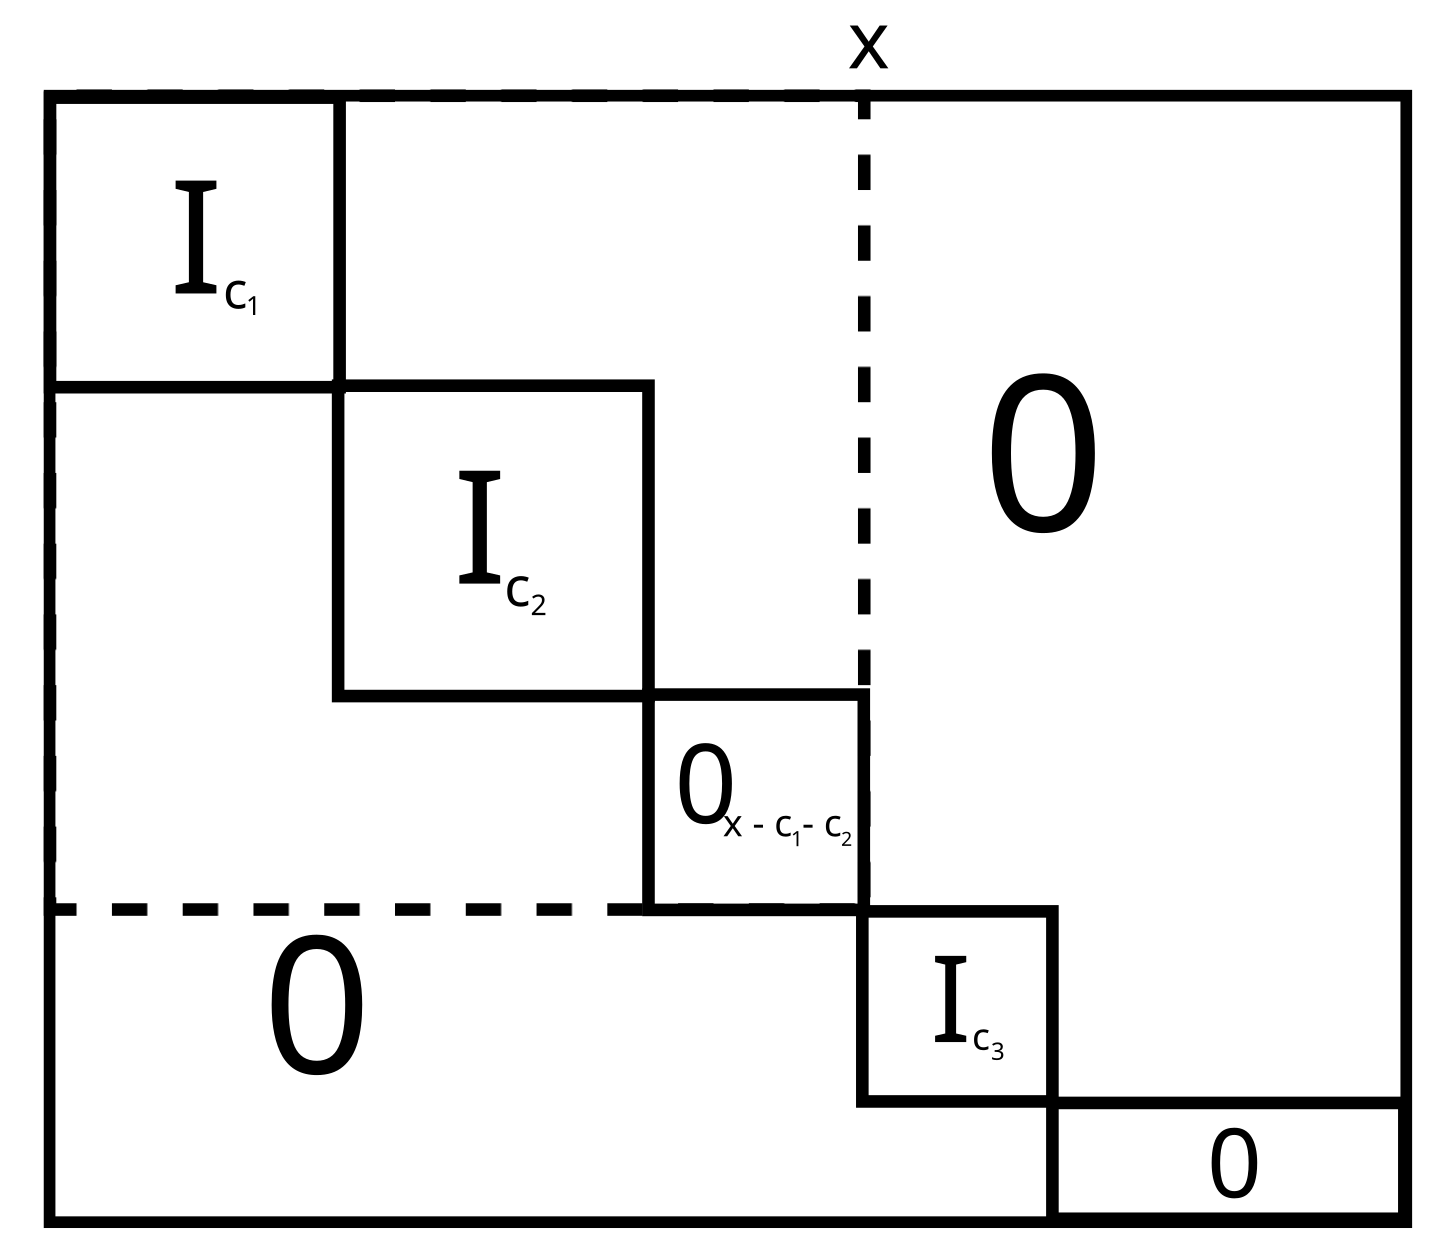
\includegraphics[scale=0.6]{matrix.png} \\
\end{center}
Рассмотрим 4 случая:
\begin{enumerate}
    \item $y \ge x, y$:

    В этом случае $c_1 = 0, c_2 = z-y+x, c_3 = y - x$.
    \item $x \ge y, z$:

    В таком случае $c_1=x - y,c_2 = y + z - x, c_3 = 0$.
    \item $z \ge x, y, \ (x + y + z) \divides 2$:

    В этой ситуации $c_1 = \frac{x + z - y}{2},c_2 = 0,c_3=\frac{y +z-x}{2}$.
    \item $z \ge x, y, \ (x + y + z) \ \cancel{\divides} \ 2$:

    В данном случае $c_1 = \frac{z + y - x - 1}{2},c_2 = 1, c_3 = \frac{x + z - y - 1}{2}$.

\end{enumerate}
Проверка сохранения всех расстояний и корректности размеров матриц (целые неотрицательные числа) очевидна, и остаётся в качестве упражнения любопытному читателю.
\end{proof}

Напомним определение $G_{m \times n}^{(k)}(\mathbb{F}) = (V_{m \times n}^{(k)}, E_{m \times n}^{(k)})$ — это граф, вершинами которого являются всевозможные матрицы размера $m \times n$ над полем $\mathbb{F}$, и две матрицы $A$ и $B$ соединены ребром, если $rk(A - B) = k$. Дальнейшие рассуждения будут посвящены этому графу.

Мы будем исследовать функцию $N(\sigma)|\sigma \in \mathcal{P}(V_{m \times n}^{(k)})$ на этом графе, равную $\{X \in V_{m \times n}^{(k)} : \forall Y \in \sigma ((X, Y) \in E_{m \times n}^{(k)})\}$ — множество всех вершин, соединённых со всеми из множества.

\begin{theorem}
Для $|\mathbb{F}| \ge 4$, $A, B \in G_{m \times n}^{(k)}(\mathbb{F})$, и $A$ и $B$ смежны, $1 < k < \min(m,n)$,
$N(N(\{A, B\})) = \{A, B\}$.
\end{theorem}
\begin{proof}
Заметим, что применение автоморфизма $X \rightarrow PXQ - R$, где $P$ и $Q$ — обратимые матрицы соответствующего размера, а $R$ — любая матрица $m \times n$, не меняет расстояние между матрицами, поэтому мы можем считать, что $A = 0, B = E_{1, 1}$.


Пусть $C \in N(N(\{A, B\})), C \ne 0$, и $C$ выглядит как \[
\left[
\begin{array}{c|ccc}
\alpha & \phantom{0} & C' & \phantom{0} \\ 
\hline \\
C_2 & \phantom{0} & C_1 \\
\phantom{0}
\end{array}
\right].
\]
где $C_1$ имеет размер $(m - 1) \times (n - 1)$. Докажем, что $C = B$ от противного. 

\textbf{Случай 1:} $rk(C) \ge 2$.

Если $C_1 = 0,$ то $C' \ne 0$ (иначе ранг $C$ будет равен 1). В таком случае мы можем применить ещё один автоморфизм на графе, который прибавляет первую строку ко второй (он не меняет ранги, поэтому всё хорошо). При этом у нас изменится матрица $B$, но это, как будет видно дальше, не повлияет на доказательство.

    В таком случае мы можем рассмотреть матрицу \[
D = 
\left[
\begin{array}{c|ccc}
\beta & \phantom{0} & 0 & \phantom{0} \\ 
\hline \\
C_2 & \phantom{0} & D_1 \\
\phantom{0}
\end{array}
\right].
\]
где $\beta \ne 0, 1, \alpha$, $rk(D_1) = k - 1, rk(D_1 - C_1) \ge k$. Тогда несложно заметить, что $D \in N(\{A, B\})$, но $rk(D - C) > k$. Противоречие.

\textbf{Случай 2:} $rk(C) = 1$.

Докажем, что $rk(B - C) \le 1$. Предположим обратное. Тогда $B = e \cdot f^T$, $C = x \cdot y^T$
 (это их скелетное разложение). Тогда по предположению векторы $e$ и $x$ линейно независимы, векторы $f$ и $y$ линейно независимы. Тогда мы можем дополнить сумму $2e \cdot f^T + x \cdot y^T$ $k-2$ слагаемыми до ранга $k$. Тогда полученная матрица, очевидно, лежит в $N(\{A, B\})$, но $rk(D - C) > k$. Противоречие.

Итак, теперь мы доказали, что $C_1 = 0$ и либо $C_2 = 0$, либо $C' = 0$. Будем считать, что $C' = 0$, второй случай доказывается аналогично. Докажем, что $\alpha = 1$ и $C_2 = 0$ от противного. Дополним $C_2$ $k-1$ л.н.з. вектором (если $C_2 = 0$, то просто возьмём $k - 1$ л.н.з. вектор) и положим их в матрицу $D_2$ (а остальное место заполним нулями). И рассмотрим матрицу \[
D = 
\left[
\begin{array}{c|ccc}
\alpha & \phantom{0} & 0 & \phantom{0} \\ 
\hline \\
C_2 & \phantom{0} & D_2 \\
\phantom{0}
\end{array}
\right].
\]
Тогда мы опять получили $D \in N(\{A, B\})$, но при этом $rk(D - C) = k - 1$. Противоречие.
Что и требовалось доказать!
\end{proof}

\begin{theorem}
    Для $|\mathbb{F}| \ge t + 3$, $A, B \in G_{m \times n}^{(k)}(\mathbb{F})$, и $d(A, B) \le k$, $1 < k < \min(m,n)$,  
    $N(N(\{A, B\})) = \{A, B\}$.
\end{theorem}
\begin{proof}
Пусть $C \in N(N(\{A, B\})), C \ne 0$ и $C$ выглядит как \[
\left[
\begin{array}{c|c}
C' & C_1 \\ 
\hline 
C_2 & C_3 \\
\end{array}
\right],
\]
где $C'$ имеет размер $t \times t$.
\begin{lemma}
    
В условиях теоремы 6 покажем, что, если $A = 0$ и \[ B = 
\left[
\begin{array}{c|c}
I_t & 0 \\ 
\hline 
* & 0 \\
\end{array}
\right],
\] то $C_3 = 0$ от противного.
\end{lemma}
\begin{proof}
    
Выберем $\alpha \ne 0, 1$ так, чтобы $\alpha$ не было собственным значением $C'$. Это возможно из-за ограничения на размер $\mathbb{F}$. Также, используя вывод из теоремы 4, выберем $D'$ так, чтобы $rk(D') = d(0, D') = k - t$, $d(C_3, D') > k - t$. Тогда рассмотрим матрицу 
\[D = 
\left[
\begin{array}{c|c}
\alpha \cdot I_t & 0 \\ 
\hline 
C_2 & D' \\
\end{array}
\right].
\]
 Несложно заметить, что $D \in N(\{A, B\})$, но 
\[d(D, C) = rk
\left(
\left[
\begin{array}{c|c}
\alpha \cdot I_t - C' & -C_1 \\ 
\hline 
0 & D' - C_3 \\
\end{array}
\right]
\right) > k.
\]
Противоречие.

P.S. Заметим, что одна из размерностей $C_1$ может быть равна 0. Тогда нужно проделать аналогичное рассуждение с $C_2$.
\end{proof}
Заметим, что применение автоморфизма $X \rightarrow PXQ - R$, где $P$ и $Q$ — обратимые матрицы соответствующего размера, а $R$ — любая матрица $m \times n$, не меняет расстояние между матрицами, поэтому мы можем считать, что $A = 0, B = I_t$.

Мы уже показали, что $C_3 = 0$. Пусть $C_1 \ne 0$. Пусть тогда в $C_1$ $j$-я строка не равна нулю. Тогда применим автоморфизм над $M_{m \times n}$, который прибавляет $j$-ю строку к $t + 1$-й. Он, очевидно, не меняет расстояние между матрицами. Тогда мы получаем противоречие с леммой 7. Аналогично $C_2 = 0$.

Пусть теперь $C'$ имеет вид 
\[
\begin{pNiceMatrix}[nullify-dots]
c_1 & \phantom{0} & K \\
\phantom{0} & \Ddots & \phantom{0} \\
L & \phantom{0} & c_t
\end{pNiceMatrix}
\]
Для начала докажем, что $\forall i \ c_i = 1 \lor c_i = 0$ от противного. Пусть $c_i \ne 1, 0$. тогда рассмотрим матрицу \[ D = 
\left[
\begin{array}{c|c}
\begin{pNiceMatrix}[nullify-dots]
c_i & \phantom{0} & 0 \\
\phantom{0} & \Ddots & \phantom{0} \\
L & \phantom{0} & c_i
\end{pNiceMatrix} & 0 \\ 
\hline 
0 & I_{k - t} \\
\end{array}
\right],
\]
Тогда очевидно, что $D \in N(\{A, B\})$, но $rk(D - C) < k$.
Получили противоречие. 

Теперь покажем, что $K = L = 0$. Опять же от обратного. Пусть $C'_{i, j} \ne 0$. Тогда мы можем применить автоморфизм, который прибавляет $j$ столбец к $i$ с коэффициентом $\beta$ таким, чтобы $\beta \cdot C'_{i, j} + C'_{i, i} \ne 1, 0$, после чего вычитает из $j$-й строчки $i$-ю с коэффициентом $\beta$. Очевидно, что он не меняет расстояние между матрицами и переводит $A$ в $A$ и $B$ в $B$. Но у матрицы, в которую перейдёт $C$, на диагонали будут не только 1 и 0. Противоречие с предыдущими рассуждениями.

И наконец покажем, что на диагонали $C'$ не может быть нулей. Если они там есть, то, так как $C \ne 0$, в $C'$ если либо блок 
\[
\left[
\begin{array}{cc}
    1 & 0 \\
    0 & 0
\end{array}
\right], 
\] либо блок 
\[
\left[
\begin{array}{cc}
    0 & 0 \\
    0 & 1
\end{array}
\right]. 
\]

Второй случай показывается аналогично, поэтому покажем только первый. Возьмём матрицу $D = 2\cdot I_k$, но на том месте, где у $C'$ стоит блок с 0 и 1, поставим блок 
\[
\left[
\begin{array}{cc}
    -1 & -1 \\
    -1 & 0
\end{array}
\right]. 
\]
Тогда $rk(B - D) = rk(0 - D) = k \implies D \in N(\{A, B\})$, но $rk(D - C) = k - 1$. Противоречие.
Откуда $C = D$. Что и требовалось доказать!
\end{proof}

\section{Заключение}
Было проведено исследование функции общих соседей на $k$-тотальном матричном графе. После симуляции над конечными полями была выдвинута гипотеза, что $N(N(\{A, B\})) = \{A, B\}$. Данная гипотеза была впоследствии доказана при некоторых ограничениях. Несмотря на ограничения, был доказан главный случай — $d(A, B) = 1$, который показал непригодность данного метода для описания общего вида автоморфизмов на данном графе, несмотря на то, что он использовался для нахождения общего вида автоморфизмов на графах со схожей структурой.

В целом результат работы очень интересный и неожиданный, так как было изучено множество крайне похожих случаев, в частности, применение этой функции на матричных графах, в которых вершины были связаны в случае обратимости разности и случай, когда матрицы $A$ и $B$ соединены ребром если $rk(A - B) \le k$, см.~\ref{lit} и~\cite{art3}, и во всех них ответ при $d(A, B) = 1$ кардинально отличался от всех остальных случаев, что выделяет полученный мной результат.

\bibliographystyle{plainurl}
\bibliography{bibl}
\end{document}